\documentclass{standalone}
\usepackage{pgfplots}
\pgfplotsset{compat=1.17}
\begin{document}
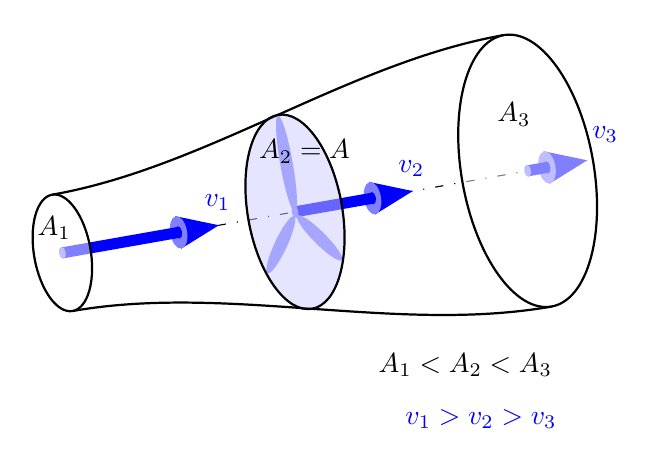
\begin{tikzpicture}[
bluedisc/.style={thick,fill=blue!20!white},
rest/.style={thick},
middleline/.style={loosely dash dot},
windarrow/.style={line width=4pt, blue}]

\begin{scope}[rotate=10]

\colorlet{bluedisc}{blue!20!white}
\colorlet{lightblue}{blue!50!white}

\draw[middleline] (0,0) -- (6,0);
\draw[rest] (0,0.75) .. controls (2,0.75) and (4,1.75) .. (6,1.75);
\draw[rest] (0,-0.75) .. controls (2,-0.75) and (4,-1.75) .. (6,-1.75);

\filldraw[blue] (2,0) -- (1.5,.2) -- (1.5,-.2) -- cycle;
    \filldraw[lightblue] (1.5,0) ellipse (.1 and .2);
    \draw[windarrow] (0,0) -- (1.5,0);
    \filldraw[lightblue] (0,0) ellipse (1pt and 2pt);
    \filldraw[blue] (1.5,0) ellipse (1pt and 2pt);
    \draw[windarrow] (0,0) (2,0) node[above] {$v_1$};
    
\filldraw[blue] (4.5,0) -- (4,0.2) -- (4,-0.2) -- cycle;
    \filldraw[lightblue] (4,0) ellipse (.1 and .2);
    \draw[windarrow] (3,0) -- (4,0);
    \filldraw[lightblue] (3,0) ellipse (1pt and 2pt);
    \filldraw[blue] (4,0) ellipse (1pt and 2pt);
    \draw[windarrow] (3,0) (4.5,0) node[above] {$v_2$};

\filldraw[blue] (6.75,0) -- (6.25,0.2) -- (6.25,-0.2) -- cycle;
    \filldraw[lightblue] (6.25,0) ellipse (.1 and .2);
    \draw[windarrow] (6,0) -- (6.25,0);
    \filldraw[lightblue] (6,0) ellipse (1pt and 2pt);
    \filldraw[blue] (6.25,0) ellipse (1pt and 2pt);
    \draw[windarrow] (6,0) (7,0) node[above] {$v_3$};

% Turbine
\fill[blue!50!white] (3,0.62) ellipse (.08 and 0.62);
\fill[blue!50!white,rotate around={35:(3.25,-0.38)}] (3.25,-0.38) ellipse (.08 and 0.4);
\fill[blue!50!white,rotate around={-35:(2.75,-0.38)}] (2.75,-0.38) ellipse (.08 and 0.4);

% Ellipse
\draw[rest,fill=white,fill opacity=.5] (0,0) ellipse (.36 and .75);
\draw[rest,fill=bluedisc,fill opacity=.5] (3,0) ellipse (.6 and 1.25);
\draw[rest,fill=white,fill opacity=.5] (6,0) ellipse (0.84 and 1.75);

\draw (0,0.6) node[anchor=north] {$A_1$};
\draw (3.3,1) node[anchor=north] {$A_2=A$};
\draw (6,1) node[anchor=north] {$A_3$};

\draw (6,-2.5) node[anchor=east] {$A_1 < A_2 < A_3$};
\draw[windarrow] (6,-3.2) node[anchor=east] {$v_1 > v_2 > v_3$};

\end{scope}
\end{tikzpicture}
\end{document}